\section{Tilstandsovergangsbetingelsar}
\thispagestyle{fancy}

For at tilstandsmaskina skal få lov til å endre tilstand, må nokre spesefikke betingelsar vere oppfylt.
Fleire av betingelsane er tidsstyrte, og alle desse tidene er justerbare via parameter.\newline
For å kunne gi ei klarare framstilling av logikken har vi valt å presentere betingelsane grafisk.
Vi har utarbeidd eit skjema som dokumenterer alle overgangsbetingelsane i tilstandsmaskina.\newline \newline

\begin{figure}[htbp]
    \centering
    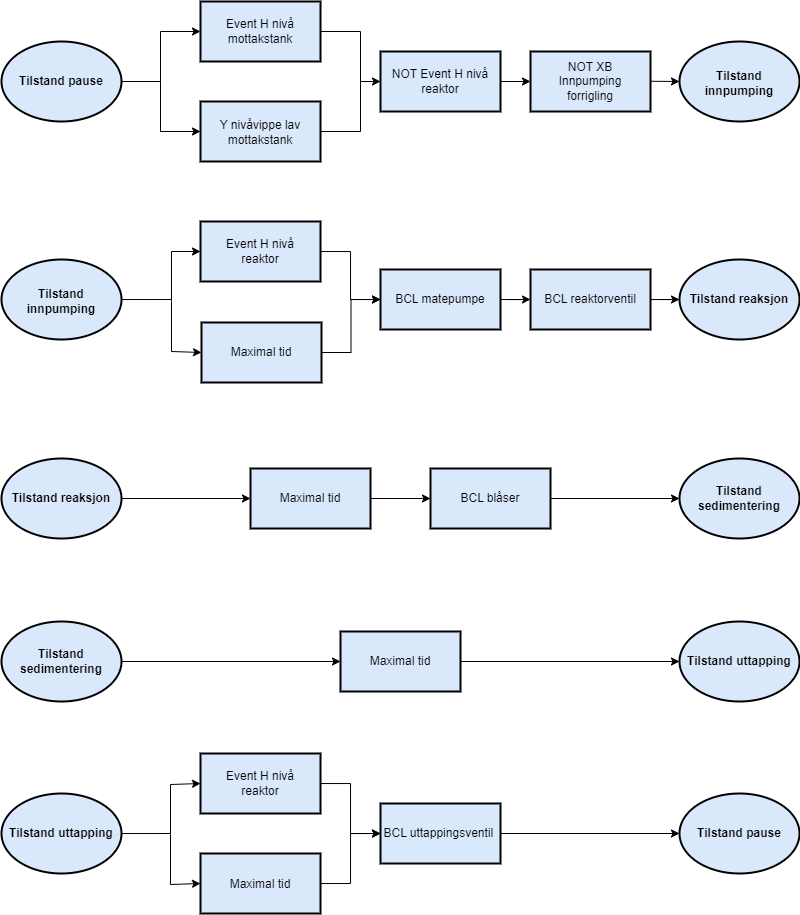
\includegraphics[scale=0.5]{Figurar/Tilstandsovergang.drawio.png}
    \caption{Grafisk presentasjon av overgangsbetingelsar}\label{fig:Tilstandsovergangsbetingelsar}
\end{figure}

\newpage